\subsection{Calibration} 

    \todoNow{Add matrix plot of LFC data}

    The calibration is needed to map each pixel on the CCD to a specific wavelength. Such a map is refered to as a wavelength solution. To do this, we need a light source with known frequencies, preferably many discret peaks. EXPRES uses a Thorium Argon lamp for an initial trial wavelength solution and a laser frequency comb (LFC) for an more precise solution.
    
    The Thorium Argon lamp produces 4,000 lines across 82 orders, which can be identified and mapped to a wavelength through a \emph{line atlas}. An intial wavelength solution for all pixels is then produced by linear interpolation. (I this project I have not done this calibration).

    The LFC generates a series of equadistant (evenly spaced) spectral lines, typically 20,000 lines across 50 orders. The range of the LFC is thus shorter, and for this reason the ThAr exposures can also be used for a rough calibration outside the LFC range. The frequencies of the LFC peaks are given by the relation
    
    \begin{equation}
        \label{eq:LFC_freq_eq}
        v_{n}=v_{\text{rep}} \times n+v_{\text{offset}}
    \end{equation}

    for integers $n$. The repetition rate $v_{\text {rep }}$ and offset frequency $v_{\text {offset }}$ are referenced against a GPS-disciplined quartz oscillator, providing calibration stability corresponding to a fractional uncertainty of less than $8 \times 10^{-12}$ for integration times greater than $1 \mathrm{~s}$. (p. 8, \cite{first_RV_from_EXPRES}). The values I have used in the calibration, $v_{\text{rep}} = 14e9$ and $v_{\text{offset}} = 6.19e9$, were provided by Lars Buchhave, but may be outdated. 

    The following procedure is followed to determine the location of the LFC peaks on the CCD: 1) Find peaks using scipy peak finding algorithm, 2) make data slices around each peak with the size of the average distance between peaks, 3) using iminuit do a $\chi^2$ minimisation fit to each peak with a super-gauss plus a linear background.

    A super-gauss, defined in eq. (\ref{eq:LFC_super_gauss}), is a regular gaussian but with an extra parameter, here denoted $P$, that allows the top of the gaussian to be flattened. The last two terms here add a linear background and an offset. 
    
    \begin{equation}
        \label{eq:LFC_super_gauss}
        f(x ; A, B, C, P, \mu, \sigma) = A \exp \left(-\left(\frac{\left(x-\mu\right)^{2}}{2 \sigma^{2}}\right)^{P}\right) + B(x-\mu) + C
    \end{equation}

    The fit then is a minimisation of  

    \begin{equation}
        \label{eq:chi2_super_gauss}
        \chi^{2}=\sum_{i=1}^{N}\left[\frac{y_{i}-f(x ; A, B, C, P, \mu, \sigma)}{\sigma_{i}}\right]^{2}
    \end{equation}

    Where $N$ is the number of peaks, $x$ is pixel-space, $y_i$ and $\sigma_i$ is the measured photon count and uncertainty respectively. The fit returns the values and uncertainties for the parameters $A, B, C, P, \mu, \sigma$ when the value of $\chi^2$ is minimized.

    \todoNow{Add plot of super-gauss fit}
    
    We are most interested in $\mu$, which gives the position of the LFC peak on the CCD (in pixel-space). With the intial rough wavelength solution dervied from the ThAr lamp (precalculated in the data set that I've used) I can determine what the approximate wavelength of the LFC peak should be. To find the better wavelength solution I then go look up the closest frequency given by eq. \ref{eq:LFC_freq_eq}. And we now have a map of ~20,000 points on the CCD with a good wavelength solution. 
    
    Of course we need to have a wavelength solution for all points on the CCD and to do that I have explored two approaches: cubic interpolation and polynomial fittting. I can evaluate the quality of the interpolation calibration by choosing to omit every second peak from the interpolation and then computing the residuals between the omitted peaks and the resulting interpolation function. For the polynomial, I can compute residuals simply by subtracting the location peaks from the fit function. Residuals from the two methods are compared in figure \ref{fig:calib_poly_vs_interp}.

    \begin{figure}[ht]
        \centering
        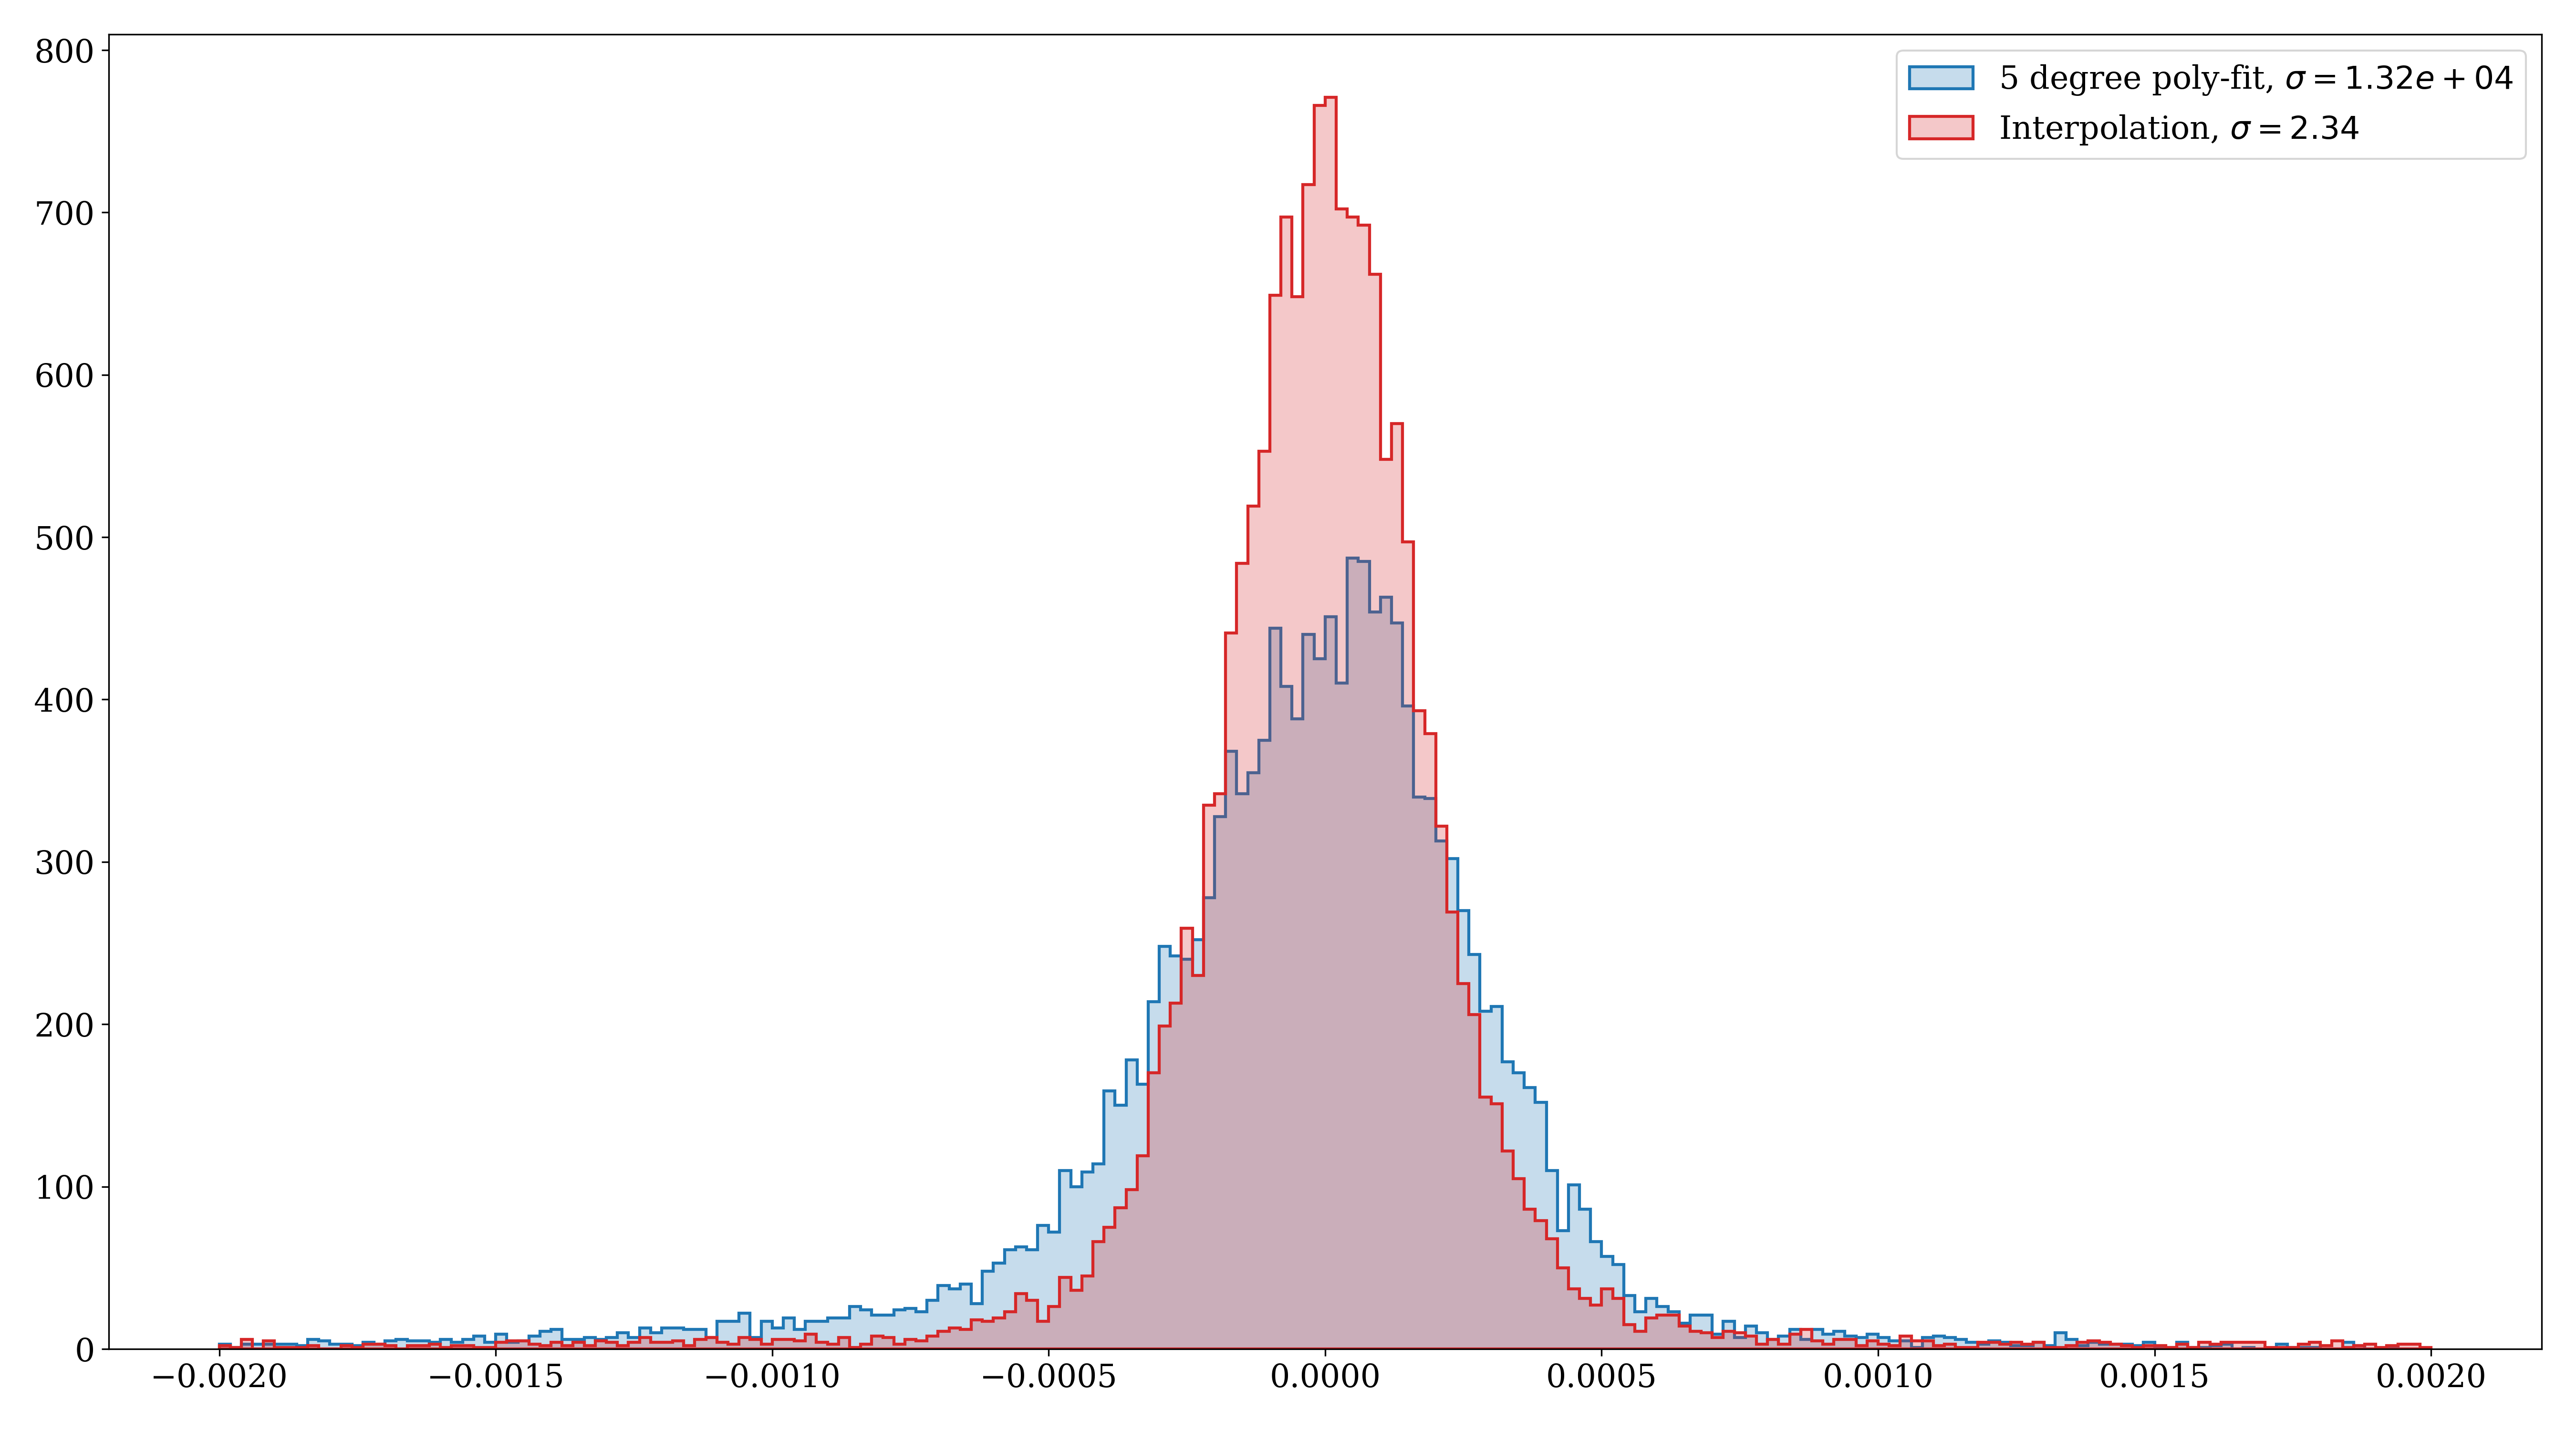
\includegraphics[scale=0.40]{figures/hist_peak_residuals_poly_and_interp.png}
        \caption{Residuals from calibrations performed through poly-fit and interpolation. Both results contain approximately the same amount of points, but the poly-fit has a much larger spread and therefore appears smaller. \todo{polyfit has 18373 lines, interp has 16888. Why? } Might be because I only use order 40-76 in the interp and all orders with more than 10 peaks for the polyfit. \todoNow{Do new polyfit calib} \todo{find out x units}}
        \label{fig:calib_poly_vs_interp}
    \end{figure}

    The standard deviation of the residuals from the interpolation come out much smaller than that of the polyfit (values specified in figure \ref{fig:calib_poly_vs_interp}), in this example, suggesting that the interpolation method is superior. It is also worth noting that because the interpolation was done on only half the data points, it will be even better when performed on all data points. A similar comparison was done to determine that the polynomial fit got better with increasing degrees until 5th. \todo{specify what file?}

    \vspace{0.5cm}

    \todo{add graph comparing residuals using gauss vs super gauss}

    \todo{perhaps add plot of changes in parameters across the CCD}

    \todo{specify run times for calibration using poly fit and interp}

    \subsubsection{Errors in the calibration data}

    The LFC fits files come with an uncertatiny on the photon count (spectrum). It appears however that this uncertatiny might be a bit underestimated. We can see this by plotting the $\chi^2$- and P-values for the LFC peak super-gauss fits, as done in figure \ref{fig:calib_errors}. The $\chi^2$ value should be roughly equal to the number of degrees of freedom in the fit, which is: 

    \begin{equation}
        \label{eq:ndof}
        N_\text{dof} = N_\text{data-points} - N_\text{fit-parameters} =  13 - 5 = 8.
    \end{equation}

    The number of data points per fit I set to be the rounded average distance bewteen peaks in a given order. Although the LFC should generate equadistant peaks, this does vary bewteen 13 and 18 points as we go through orders, most fits having 13 data points (see figure \ref{fig:N_data_points} in \ref{appendix:LFC_errors}). We should therefore see a spike in the $\chi^2$ values roughly around 8, falling of at a slower pace to the right side. Looking again at figure \ref{fig:calib_errors}, this is not the case for the errors as provided (scale-factor 1). But multiplying by $\sqrt{3}$ we get much closer. $\sqrt{10}$ is overdoing it, however. I looked at several other scaling factors bewteen $\sqrt{3}$ and $\sqrt{10}$, see figure \ref{fig:calib_errors_extensive} in \ref{appendix:LFC_errors} for details, and $\sqrt{3}$ comes closest to giving a peak at 8.
    
    Another check is that the probability distribution should be roughly flat. \todo{explain why, \href{https://stats.stackexchange.com/a/481843/353364}{help}}.
    
    \begin{figure}[ht]
        \centering
        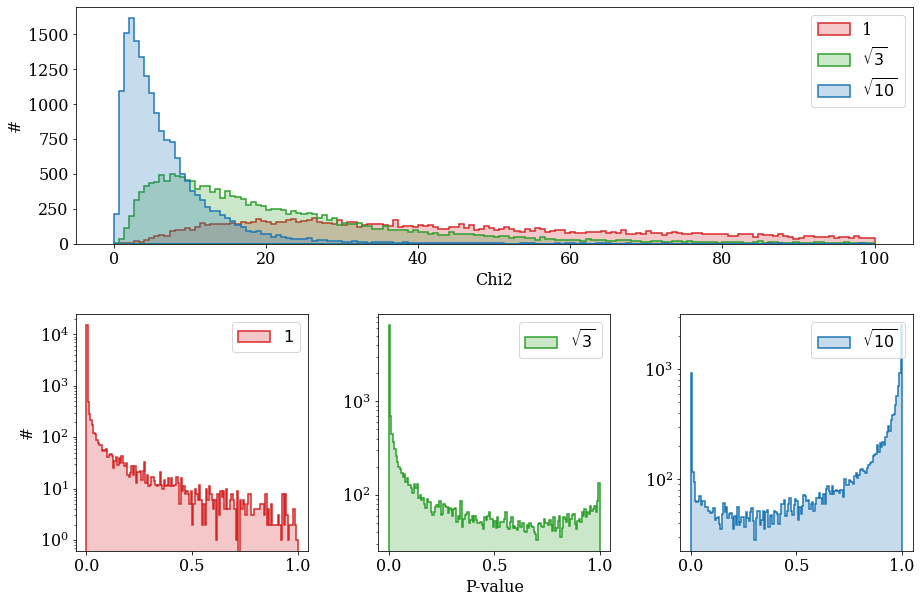
\includegraphics[scale=0.40]{figures/calib_errors.png}
        \caption{Chi2-values and P-values from individual LFC peak super-gauss fits with photon count (spectrum) errors multiplied by different scale-factors (1, $\sqrt{3}$ and $\sqrt{10}$). See text for more datails.}
        \label{fig:calib_errors}
    \end{figure}

    \todo{explain why we use factors of square-root:} Something to do with putting into the chi2 which is a square sum, so the square-root goes away. 

    \bigbreak

    \noindent \textbf{Effects on calibration:} \newline
    The errors used during the production of the calibration residuals shown in figure \ref{fig:calib_poly_vs_interp} I have already multiplied by $\sqrt{3}$. This gaves us a $\sigma = 0.934$, without this correction I got $\sigma = 2.34$. 

    \todo{Computing the sigma for different error scaling factors gave very jumpy results.. why?} 

\subsection{RV extraction}
    In my attempt to determine radial velocities (RV), I've take the following very straight forward approach: 
    \begin{itemize}
        \item First 
    \end{itemize}
    
    I've taken the very straight forward approach of fitting a shift-parameter to minimize the difference between the spectrum count for two spectra. 


    \begin{itemize}
        \item Hist fit / cross-correlation
        \begin{itemize}
            \item Order approach
            \item Feature approach
            \item (Run times)
        \end{itemize}
        \item Extracting relative radial velocities from over constraint system (Matrix reduction to circumvent correlations)
        \item Future ideas
        \begin{itemize}
            \item Auto encoder
        \end{itemize}
    \end{itemize}

